\section{Positionierungs Algorithmen}
\label{sec:algorithmen}

\begin{frame}
  \frametitle{Algorithmen - Warum nicht GPS?}

  \begin{itemize}
  \item Vorteile
    \begin{itemize}
    \item sehr genau (1 bis 3 Meter)
    \item globale Position
    \item einfach zu Implementieren
    \end{itemize}
  ~\\
  \item Probleme
    \begin{itemize}
    \item schlechter Empfang in Gebäuden
    \item hohe Kosten
    \item zu groß und schwer für einen Sensorknoten
    \item hoher Stromverbrauch
    \end{itemize}
  \end{itemize}
\end{frame}

\begin{frame}
  \frametitle{Algorithmen\footnote{Gholami, M. R. (2011). Positioning Algorithms for
      WirelessSensor Networks. Chalmers University of Technology.}}

  \begin{center}
    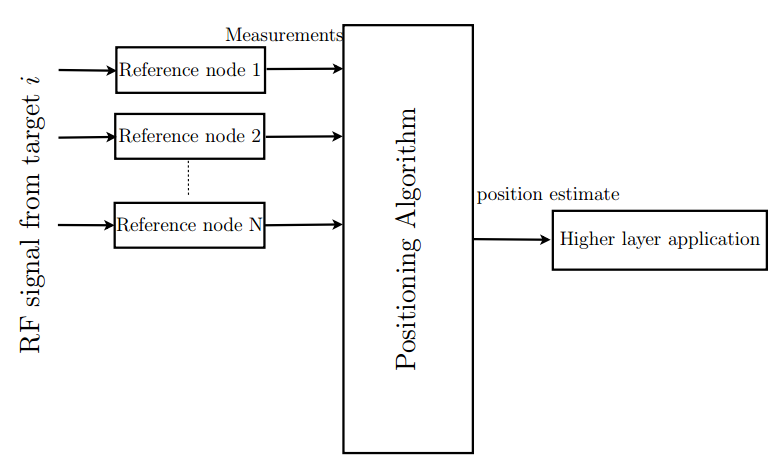
\includegraphics[scale=0.35]{img/algo_1}
  \end{center}
\end{frame}

\begin{frame}
  \frametitle{Triangulation}

  \begin{center}
    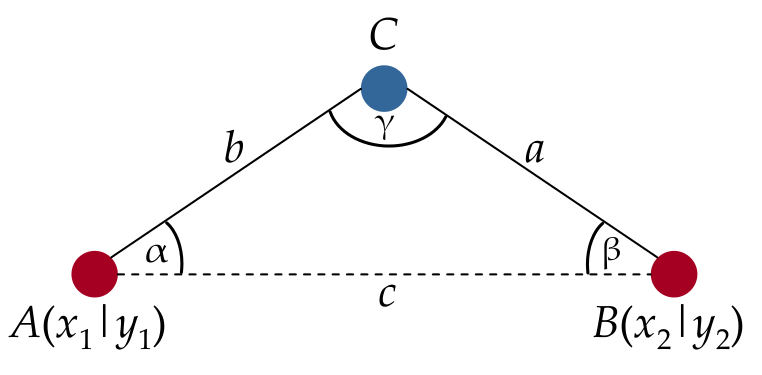
\includegraphics[scale=0.2]{img/triang}\\~\\

    $c = \sqrt{(B_{x)} - A_{x})^2 + (B_{y} - A_{y})^2}$\\
    $\varphi = arctan(\frac{B_{y} - A_{y}}{B_{x}} - A_{x})$\\
    $b = c \cdot \frac{sin(\beta)}{sin(\alpha + \beta)}$\\~\\

     \begin{tabular}{rr}
       $C_{x} = A_{x} + b \cdot cos(\varphi)$ & $C_{y} = A_{x} + b \cdot sin(\varphi)$ \\ 
     \end{tabular}
  \end{center}
\end{frame}

\begin{frame}
  \frametitle{Trilateration}

  \begin{center}
    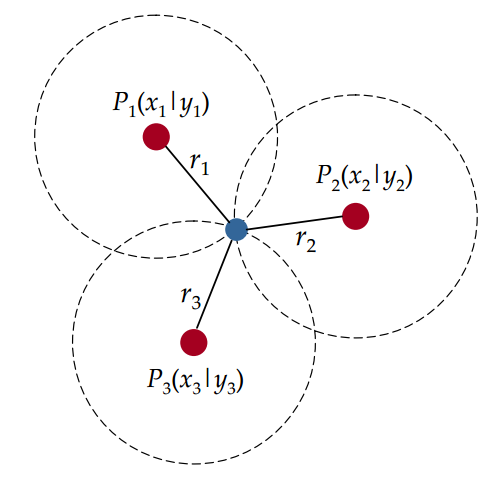
\includegraphics[scale=0.2]{img/trilat}\\~\\

    $
    \begin{pmatrix}
      P_{x} \\
      P_{y}
    \end{pmatrix}
    =
    H^{-1} \cdot z
    $\\~\\
    $
    H = 
    \begin{bmatrix}
      2 \cdot x_{1} - 2 \cdot x_{2} & 2 \cdot y_{1} - 2 \cdot y_{2} \\
      2 \cdot x_{1} - 2 \cdot x_{3} & 2 \cdot y_{1} - 2 \cdot y_{3}
    \end{bmatrix}
    $\\~\\
    $
    z = 
    \begin{pmatrix}
      r_{2}^2 - r_{1}^2 + x_{1}^2 - x_{2}^2 + y_{1}^2 - y_{2}^2 \\
      r_{3}^2 - r_{1}^2 + x_{1}^2 - x_{3}^2 + y_{1}^2 - y_{3}^2
    \end{pmatrix}
    $
  \end{center}
\end{frame}

\begin{frame}
  \frametitle{Signallaufzeitmessung (ToA)}

  \begin{center}
    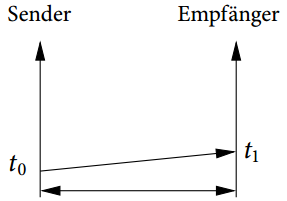
\includegraphics[scale=0.35]{img/time1}\\~\\

    $d = (t_{1} - t_{0}) \cdot c$\\~\\
    $c=299\,792\,458\;\mathrm{m/s}$
  \end{center}
\end{frame}

\begin{frame}
  \frametitle{Signallaufzeitmessung (TDoA)}

  \begin{center}
    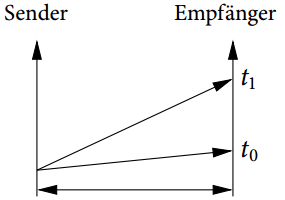
\includegraphics[scale=0.35]{img/time2}\\~\\

    $d \approx (t_{1} - t_{0}) \cdot c_{0}$\\~\\
    $c_{0}\footnote{bei 20° trockener Luft} = 343\mathrm{m/s}$
  \end{center}
\end{frame}

\begin{frame}
  \frametitle{Signallaufzeitmessung (RToF)}

  \begin{center}
    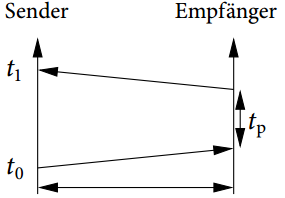
\includegraphics[scale=0.35]{img/time3}\\~\\

    $d = \frac{t_{1} - t_{2} - t_{p}}{2} \cdot c$\\~\\
    $c=299\,792\,458\;\mathrm{m/s}$
  \end{center}
\end{frame}